Динамика количества атомов в МОЛ:
\begin{equation*}
	\frac{d N}{d t} = \sub{\Phi}{load} - \cancel{\gamma N} - \beta N^2
	\hspace{0.5cm} \Rightarrow \hspace{0.5cm}
	N(t) = \sqrt{\frac{\sub{\Phi}{load}}{\beta}} \left(1-e^{-t \sqrt{\beta \sub{\Phi}{load}}}\right)
\end{equation*}




\begin{minipage}{0.6\textwidth}


\begin{figure}[h]
    \centering
    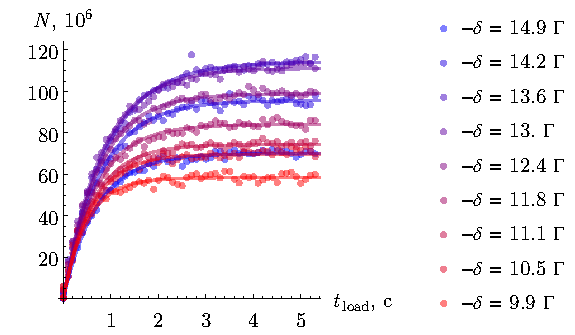
\includegraphics[width=0.8\textwidth]{../MOT/figs/motload_v2.pdf}
    \caption{Динамика загрузки МОЛ для различных значений отстройки $\delta$ лучей МОЛ}
    %\label{fig:}
\end{figure}

\end{minipage}
\hfill
\begin{minipage}{0.35\textwidth}

\begin{figure}[h]
    \centering
    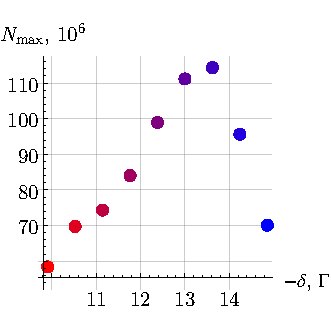
\includegraphics[width=0.8\textwidth]{../MOT/figs/motload2_v2.pdf}
    \caption{Зависимость максимального числа атомов в МОЛ от величины отстройки $\delta$ лучей МОЛ}
\end{figure}

\end{minipage}